\documentclass{beamer}
\usepackage[utf8]{inputenc}

\usepackage{semantic}
\usepackage{graphicx}
\usepackage{booktabs}
\usepackage{todonotes}
\presetkeys{todonotes}{inline}{}

\usepackage[absolute,overlay]{textpos}
% This is to get textpos to play well,
% A stackoverflow user mentioned that this could
% cause problems in some Acrobat Reader versions
% I'll take the chance
\usebackgroundtemplate{}


\mode<presentation> {
\usetheme{boxes} % When headline is wanted use Dresden theme instead
\usecolortheme{seagull}
\setbeamertemplate{footline}[page number]
\setbeamertemplate{navigation symbols}{}
}


%----------------------------------------------------------------------------------------
%	TITLE PAGE
%----------------------------------------------------------------------------------------

\title[Coding Pirates] % bottom of every slide
  {Teaching kids programming, IT-creativity and modern tech} % title page

\author{\footnotesize{Martin Dybdal} \\ \footnotesize{\texttt{dybber@dybber.dk}}}

\institute {
DIKU \\
University of Copenhagen
}

\date{5 April 2016}

\begin{document}

{
\setbeamertemplate{headline}{}
\begin{frame}
  \begin{center}
    \includegraphics[width=0.7\textwidth]{imagery/codingpirates.png}
  \end{center}
\vspace{-1cm}
\titlepage
\end{frame}
}

%----------------------------------------------------------------------------------------
%	TABLE OF CONTENTS
%----------------------------------------------------------------------------------------

\begin{frame}
\frametitle{Overview}
\tableofcontents
\end{frame}

%----------------------------------------------------------------------------------------
%	CONTENT
%----------------------------------------------------------------------------------------

\section{What is Coding Pirates?}
\begin{frame}
\frametitle{What is Coding Pirates?}
\begin{textblock}{20}(6,5)
% \includegraphics[width=0.4\textwidth]{imagery/william-sofie}
 %\includegraphics[width=\textwidth]{imagery/cpthack-and-miss1337-transp.png}
\end{textblock}

\begin{itemize}
\item Activity for kids aged 7-17 years
\item A playground - not just two more hours of school
\item An attempt to change the school system
\end{itemize}

\begin{center}
   \includegraphics[width=0.6\textwidth]{imagery/william-sofie}
\end{center}

\end{frame}

\subsection{Who are Coding Pirates?}
\begin{frame}
\frametitle{Who are Coding Pirates?}
\begin{itemize}
\item Non-profit organisation
\item +250 volunteers in Coding Pirates network
  \begin{itemize}
  \item Teachers, IT professionals, researchers, librarians, IT students
  \end{itemize}
\item 30 hubs in Denmark
\item $\sim$700 paying members
\end{itemize}

\centerline{\includegraphics[width=0.9\textwidth]{imagery/gamejam}}
\end{frame}

\subsection{Why Coding Pirates?}

\begin{frame}
\frametitle{Why Coding Pirates?}

\begin{textblock}{16}(0,2)
{
\setlength{\fboxsep}{0pt}%
\setlength{\fboxrule}{1pt}%
\only<2>{\centerline{\fbox{\includegraphics[width=0.5\textwidth]{imagery/ugebreveta4-automatisering}}}}
\only<4>{\centerline{\fbox{\includegraphics[width=0.5\textwidth]{imagery/transcriptic-workcell}}}}
%\only<4>{\centerline{\fbox{\includegraphics[width=0.5\textwidth]{imagery/skat-efi}}}}
%\only<6>{\centerline{\fbox{\includegraphics[width=0.7\textwidth]{imagery/ip_allplots}}}}
%\only<7>{\centerline{\fbox{\includegraphics[width=0.5\textwidth]{imagery/toiletpaper-carousel}}}}
}
\end{textblock}

\only<1-5>{
\begin{itemize}
\item Computational thinking - a 21st century skill
\item Automatisation
\item Democracy: New tech requires new policies. The public
  should be able to make informed decisions
\end{itemize}
}

\only<6>{
\begin{center}
  \huge Our kids needs to be IT-productive, not just consumers.
\end{center}
}


\end{frame}

\section{Coding Pirates in practice}
\begin{frame}
\frametitle{In practice}

\begin{textblock}{20}(8,0.5)
 \includegraphics[width=0.3\textwidth]{imagery/scratch}
\end{textblock}

\begin{textblock}{20}(6,9)
  \includegraphics[width=0.4\textwidth]{imagery/arduino-theremin}
\end{textblock}

\begin{itemize}
\item $\sim$25-30 kids
\item $\sim$7-10 volunteers
\item 2 hours a week, usually 17:00-19:00
\item 15 minutes break with snacks, cool aid, fruit etc.
\item Bring your own device (BYOD)
\end{itemize}
\vspace{2cm}

\end{frame}

\begin{frame}
\frametitle{Workshops}

\begin{itemize}
\item 4-6 week workshops
  \begin{itemize}
  \item Scratch
  \item LEGO Mindstorms
  \item 3D printing
  \item Processing
  \item Arduino
  \item Unity
  \item 3D modelling in Blender
  \end{itemize}
\item Kids can not switch between workshops during these 4-6 weeks
\item Presentations at the end of a 4-6 week period
\end{itemize}

\end{frame}

% \begin{frame}
%  \vspace{5mm}
%  \includegraphics[width=\textwidth]{imagery/codingpirates-diku}
% \end{frame}

% \begin{frame}
%  \vspace{5mm}
%  \includegraphics[width=\textwidth]{imagery/william-sofie}
% \end{frame}

\begin{frame}
 \vspace{5mm}
 \includegraphics[width=\textwidth]{imagery/arduino-workshop}
\end{frame}

\begin{frame}
 \vspace{5mm}
 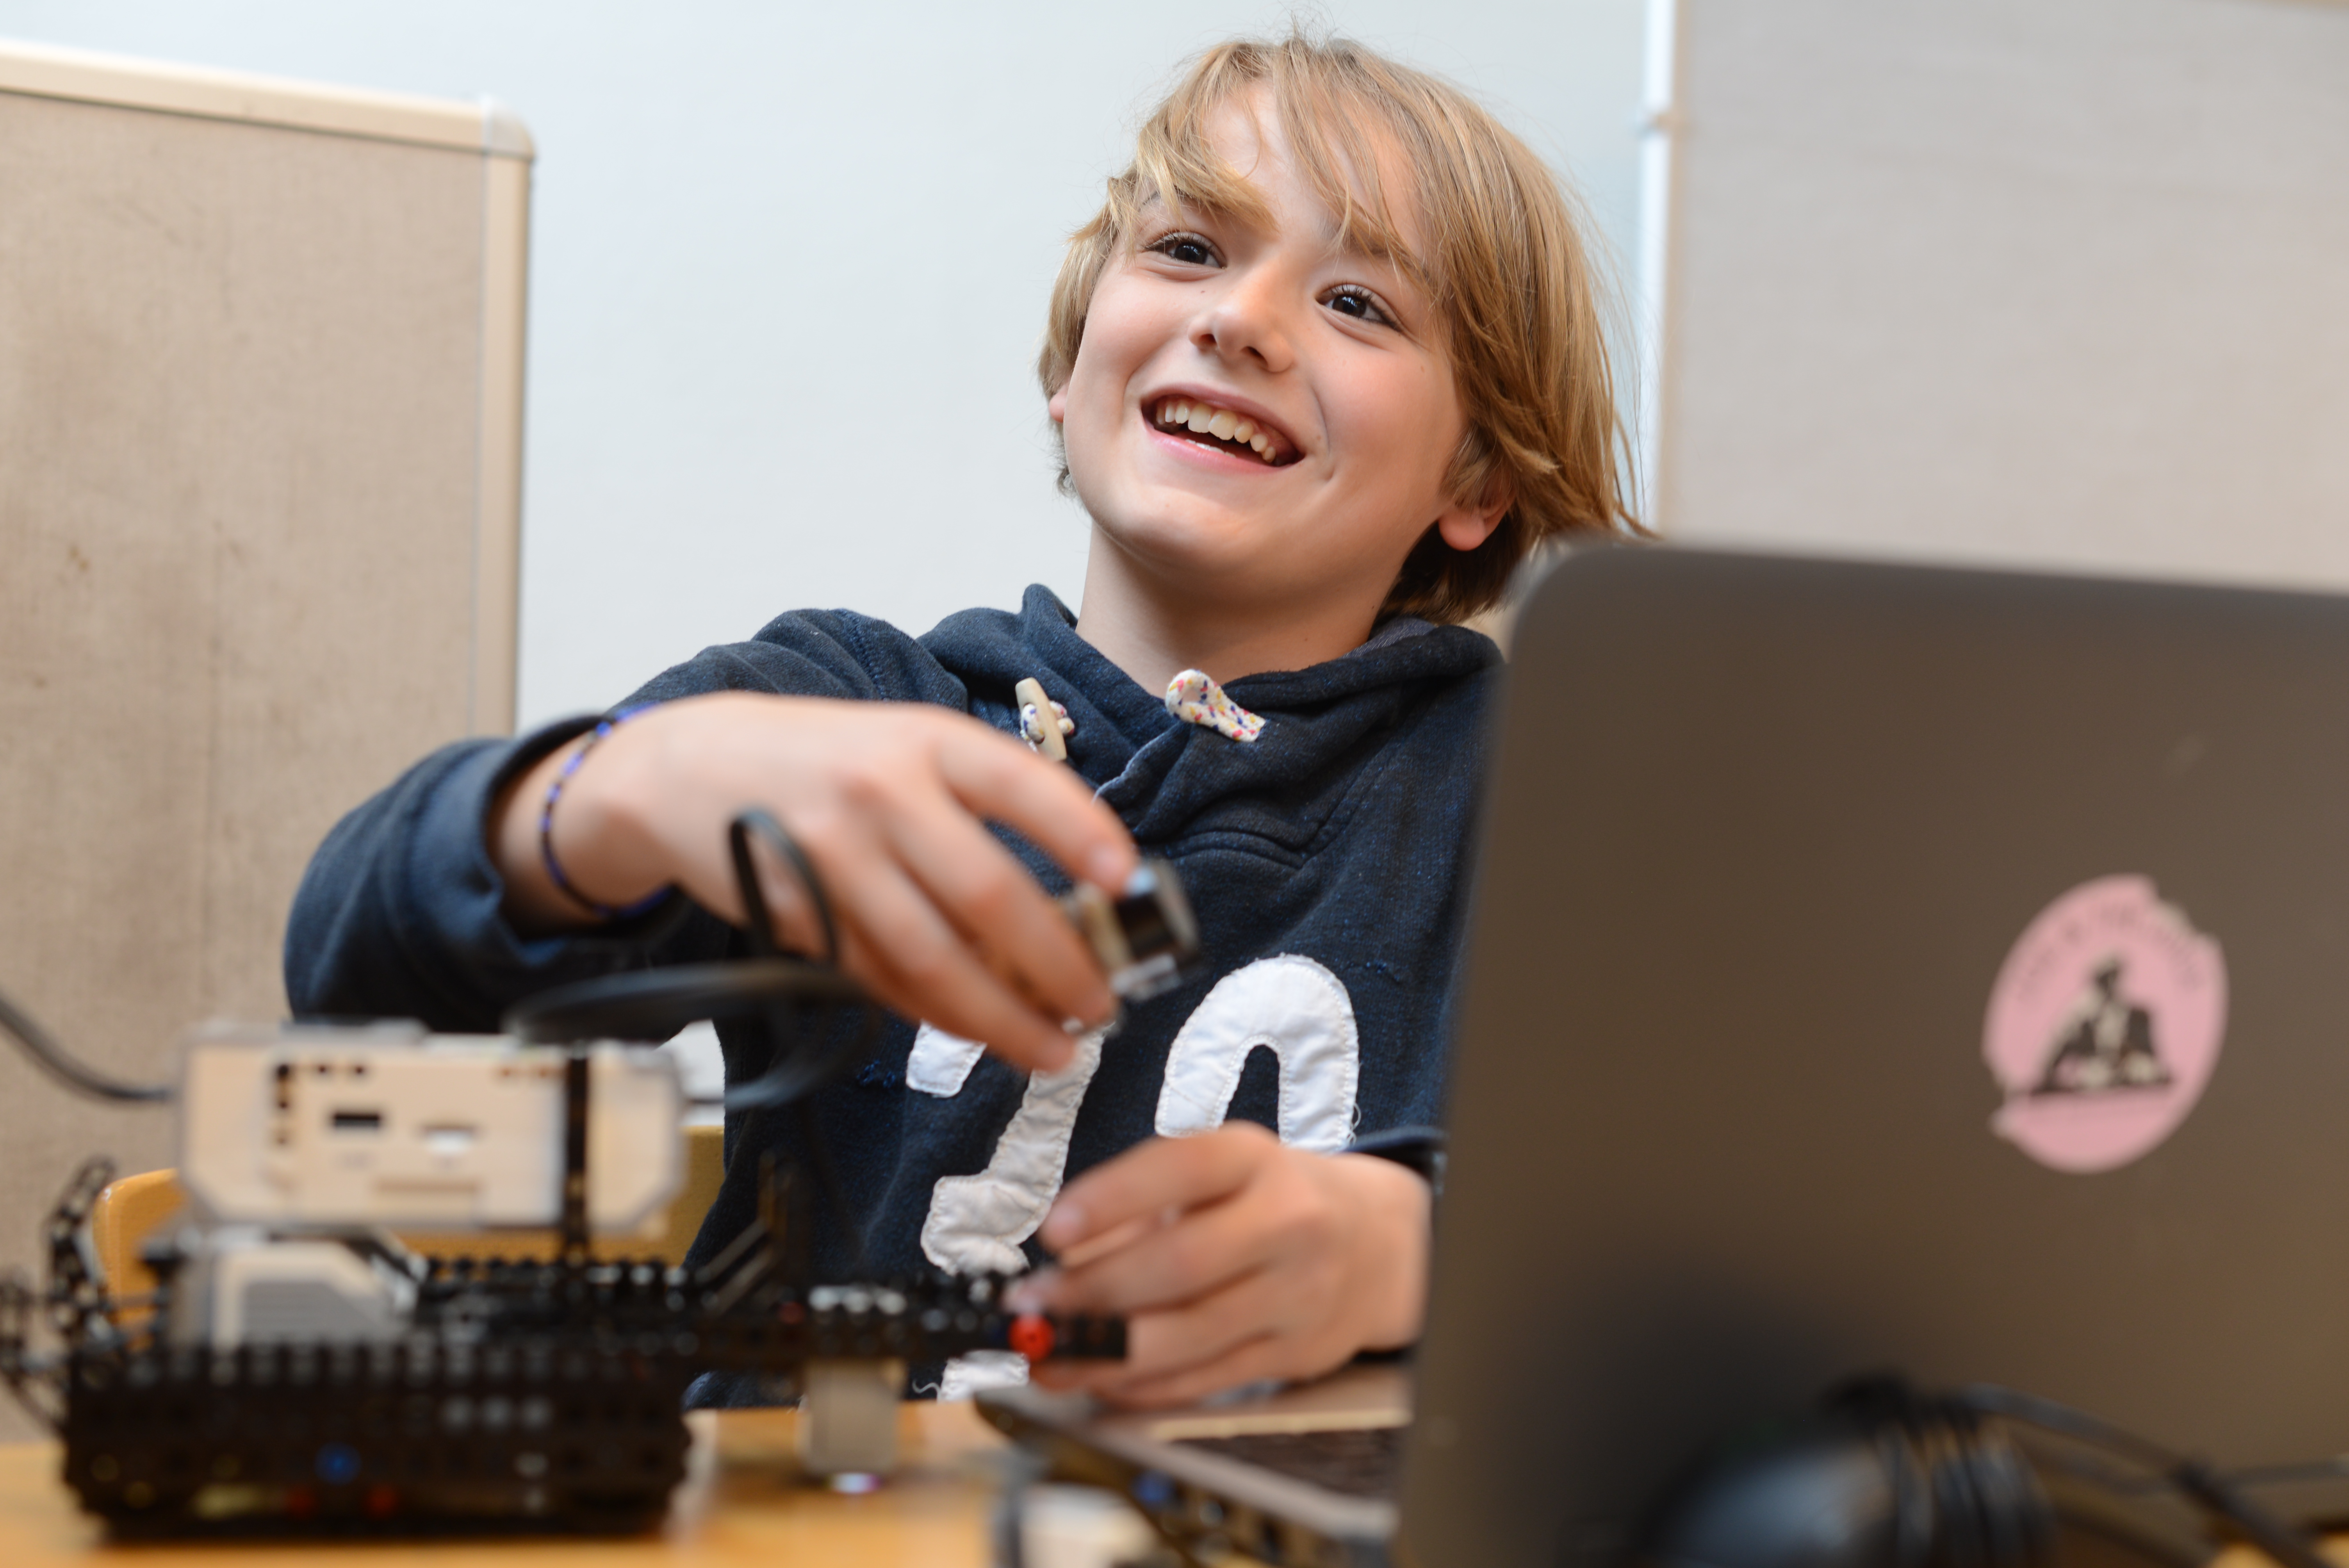
\includegraphics[width=\textwidth]{imagery/august-mindstorms}
\end{frame}

\begin{frame}
 \vspace{5mm}
 \includegraphics[width=\textwidth]{imagery/mindstorms-presentation}
\end{frame}

\subsection{Example project}

\begin{frame}
  \frametitle{Stickman dungeon}
  by Alexander and Oscar, 11 years

  \centerline{\includegraphics[width=0.8\textwidth]{imagery/stickman-dungeon}}

  \url{https://scratch.mit.edu/projects/57201286/}
\end{frame}


\subsection{Philosophy}
\begin{frame}
\frametitle{Philosophy}

\begin{itemize}
\item Constructionism
\item Creativity
\item Curiosity
\item Exploration
\end{itemize}

\end{frame}

% \begin{frame}
%   \frametitle{Example project: Horror teddy bear}
%   by Penelope, 12 years
%   \vspace{7mm}

%   \includegraphics[width=\textwidth]{imagery/penelope-raedselsbamse}

%   \url{https://www.youtube.com/watch?v=Mc21BbiUGxU}
% \end{frame}







% \subsection{Scratch}
% \begin{frame}
% \vspace{1cm}
%  \includegraphics[width=\textwidth]{imagery/scratch-logo}

% \end{frame}

% \begin{frame}
% \frametitle{Scratch 4 Arduino}

% \end{frame}

% \section{Processing(.js)}
% \begin{frame}
% \frametitle{Processing(.js)}

% \end{frame}

% \subsection{... and other technologies}
% \begin{frame}

% \frametitle{Other technologies used}
% \todo{find logos}

% \begin{itemize}
% \item Processing(.js) via KhanAcademy
% \item Arduino
% \item Blender (3D modelling)
% \item Unity (2D and 3D games)
% \item LEGO Mindstorms and LEGO WeDo (expensive)
% \item littleBits (expensive)
% \end{itemize}
% \end{frame}


% \begin{frame}
%   \frametitle{Robot-sumo}
%   \includegraphics[width=\textwidth]{imagery/robotsumo}
  
%   \url{https://www.youtube.com/watch?v=qcWTpXh-rOw}
% \end{frame}


% \begin{frame}
%   \frametitle{3D printed autonomous Arduino boat}
%   by Niels, 12 years

%   \vspace{2mm}
%   \centerline{\includegraphics[width=0.8\textwidth]{imagery/pasta_autonomous_submarine}}
% \end{frame}

% \begin{frame}
%   \frametitle{iOS app: ``Draw the wall''}
%   by William, 14 years

%   \vspace{2mm}
%   \centerline{\includegraphics[width=0.8\textwidth]{imagery/drawthewall}}
% \end{frame}

% \subsection{Difficulties}
% \begin{frame}
% \frametitle{Difficulties ahead}
% \begin{itemize}
% \item Few pirates from age 14 and up
% \item Few girls
% \item Fostering friendships is hard, but important
% \item Further education of volunteers
% \item Retaining and recruiting volunteers
% \end{itemize}
% \end{frame}

% \begin{frame}
%   \frametitle{Age and gender (including waiting list)}
%   \centerline{\includegraphics[width=\textwidth]{../datacrunching/age-gender-hist}}
% \end{frame}

% \begin{frame}
%   \frametitle{Percentage of girls by age (including waiting list)}
%   \centerline{\includegraphics[width=\textwidth]{../datacrunching/girl_percentage}}
% \end{frame}

% \subsection{The Coding Pirates Community}
% \begin{frame}
%   \frametitle{Volunteer community}
%   \includegraphics[width=\textwidth]{imagery/unity-for-volunteers.jpg}
% \end{frame}


% \section{Computing in schools}
% \begin{frame}
%   \frametitle{Computing in schools}
%   \begin{quotation}
%     "The computer is the Proteus of machines. Its essence is its
%     universality, its power to simulate. Because it can take on a
%     thousand forms and can serve a thousand functions, it can appeal
%     to a thousand tastes."

%     - Seymour Papert, in Mindstorms
%   \end{quotation}

%   We can already use this when teaching e.g. history, biology, chemistry,
%   or language classes!

%   \begin{itemize}
%   \item Make a game that teaches grade $N-1$ about photosynthesis
%   \item Make a game that teaches grade $N-1$ about life in ancient Rome
%   \item Make an interactive story that tells the story XYZ
%   \end{itemize}

%   More fun than a poster or a written report!
% \end{frame}

% \begin{frame}
%   \frametitle{But what do we want schools to teach?}

%   \begin{itemize}
%   \item Teach computing as a discipline, e.g. like math
%     \begin{itemize}
%     \item Algorithms vs. data
%     \item Systematic problem solving
%     \item Computational thinking
%     \end{itemize}
%   \item Teach computing as a craft/skill, e.g. like woodwork
%     \begin{itemize}
%     \item Focus on creation and tools
%     \item Creative and reflective thinking
%     \end{itemize}
%   \item A mix?
%   \item As a separate discipline or inside other classes?
%   \end{itemize}
% \end{frame}

% \section{DIKU's involvement}
% \begin{frame}
% \frametitle{Why does a university use time teaching tweens and teens?}
% \begin{itemize}
% \item Supply chain management
% \item The teachers needs our expertise
% \item Defining how computing should be taught in Schools
% \item Potential research areas
% \item Teacher education and re-education
% \item Because we have connections to potential volunteers (e.g. alumni)
% \item Good publicity and great advertisement
% \end{itemize}
% \end{frame}

% \begin{frame}
%   \centerline{\includegraphics[width=\textwidth]{imagery/brickbacker}}
% \end{frame}


% \begin{frame}
%   \frametitle{Coding Pirates in Gothenburg?}
%   \begin{center}
%     \includegraphics[origin=c,angle=-20,width=0.7\textwidth]{imagery/wanted}
%   \end{center}

% \end{frame}


% \begin{frame}
%   \frametitle{Research questions}

%   \begin{itemize}
%   \item How do we best integrate these subjects in schools and high-schools?
%   \item Can a single teacher manage?
%   \item Will we benefit from using \textit{computer games} as a medium
%     in other subjects? E.g. physics, history, music.
%   \end{itemize}

% \end{frame}

\begin{frame}
  \begin{center}
    \huge Unlocking creativity and curiosity is key when teaching
    programming.
  \end{center}

\end{frame}


\begin{frame}
\frametitle{Coding Pirates}

\begin{textblock}{15}(2,5.5)
\textbf{Coding Pirates}\\
http://codingpirates.dk\\
kontakt@codingpirates.dk\\ ~
\\
\textbf{Martin Dybdal}\\
University of Copenhagen\\
dybber@dybber.dk\\
%\includegraphics[width=0.4\textwidth]{imagery/codingpirates.png}
\end{textblock}


\begin{textblock}{7}(7.5,5.5)
\includegraphics[width=\textwidth]{imagery/martin}
\end{textblock}


\end{frame}


\end{document}